\documentclass[a4paper,10pt,landscape,twocolumn]{scrartcl}

%% Settings
\newcommand\problemset{11}
\newcommand\worksession{Tuesday, 17 October 2017}
\newif\ifcomments
\commentsfalse % hide comments
%\commentstrue % show comments

%% Packages
\usepackage[english]{exercises}
\usepackage{wasysym}
\usepackage{hyperref}
\hypersetup{colorlinks=true, urlcolor = blue, linkcolor = blue}
\usepackage{enumitem}
\usepackage{graphicx}

%% Macros
\usepackage{xspace}

\newcommand{\eps}{\varepsilon}
\newcommand{\ket}[1]{|#1\rangle}
\newcommand{\bra}[1]{\langle#1|}
\newcommand{\inp}[2]{\langle{#1}|{#2}\rangle}
\newcommand{\norm}[1]{\parallel\!#1\!\parallel}
\newcommand{\points}[1]{\marginpar{\textbb{#1 p.}}}
\newtheorem{theorem}{Theorem}
\newtheorem{definition}{Definition}
\newtheorem{proposition}{Proposition}
%\newenvironment{proof}{\noindent {\bf Proof }}{{\hfill $\Box$}\\}

\newcommand{\gen}{\ensuremath{\mathsf{Gen}}\xspace}
\newcommand{\enc}{\ensuremath{\mathsf{Enc}}\xspace}
\newcommand{\dec}{\ensuremath{\mathsf{Dec}}\xspace}
\newcommand{\mac}{\ensuremath{\mathsf{Mac}}\xspace}
\newcommand{\vrfy}{\ensuremath{\mathsf{Vrfy}}\xspace}
\newcommand{\negl}{\ensuremath{\mathsf{negl}}\xspace}
\newcommand{\PrivK}{\ensuremath{\mathsf{PrivK}}\xspace}
\newcommand{\eav}{\ensuremath{\mathsf{eav}}\xspace}

\newcommand{\Z}{\ensuremath{\mathbb{Z}}}
\newcommand{\R}{\ensuremath{\mathbb{R}}}
\newcommand{\N}{\ensuremath{\mathbb{N}}}


\newcommand\floor[1]{\lfloor#1\rfloor}
\newcommand\ceil[1]{\lceil#1\rceil}

% \newcommand{\comment}[1]{{\sf [#1]}\marginpar[\hfill !!!]{!!!}}
\newcommand{\chris}[1]{\comment{\color{blue}Chris: #1}}
\newcommand{\jan}[1]{\comment{\color{magenta}Jan: #1}}




\begin{document}

\problems

{\sffamily\noindent
We will work on the following exercises together during the work sessions on \worksession.

You are strongly encouraged to work together on the exercises, including the homework. You do not have to hand in solutions to these problem sets.}


\begin{exercise}[El Gamal encryption]
As in Example 11.17 in [KL], let $\mathbb{G}$ be the subgroup of $\mathbb{Z}_{167}^*$ generated by $g=4$. We have that the order $q=|\mathbb{G}|=83$ is prime. Let the secret key be $x=23 \in \Z_{83}$ and so the public key is $pk = \langle p,q,g,h \rangle = \langle p,q,g,g^x \rangle$ 
\begin{subex}
Compute the $h$ component in the public key.
\end{subex}
\begin{subex}
Compute the encryption of message $m=19 \in \mathbb{G}$ with randomness $y=44$.
\end{subex}
\begin{subex}
Decrypt the ciphertext $\langle c_1,c_2 \rangle = \langle 132,44 \rangle$.
\end{subex}
\end{exercise}


\begin{exercise}[RSA encryption]
As in Example 11.27 in [KL], say $\mathsf{GenRSA}$ outputs $(N,e,d)=(1005973,89,d)$. Note that $1005973=997 \cdot 1009$.
\begin{subex}
Encrypt the message $m=1234 \in \Z_{1005973}^*$
\end{subex}
\begin{subex}
Compute the private key $(N,d)$ corresponding to the public key $(N,e)=(1005973,89)$.
\end{subex}
\begin{subex}
Decrypt the ciphertext $c=530339$.
\end{subex}
\end{exercise}

{
\centering
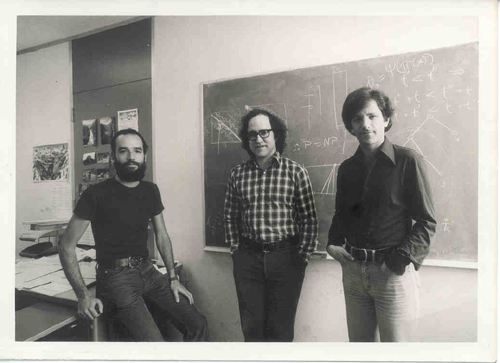
\includegraphics[height=0.15\textwidth]{RSA-MIT.jpg} 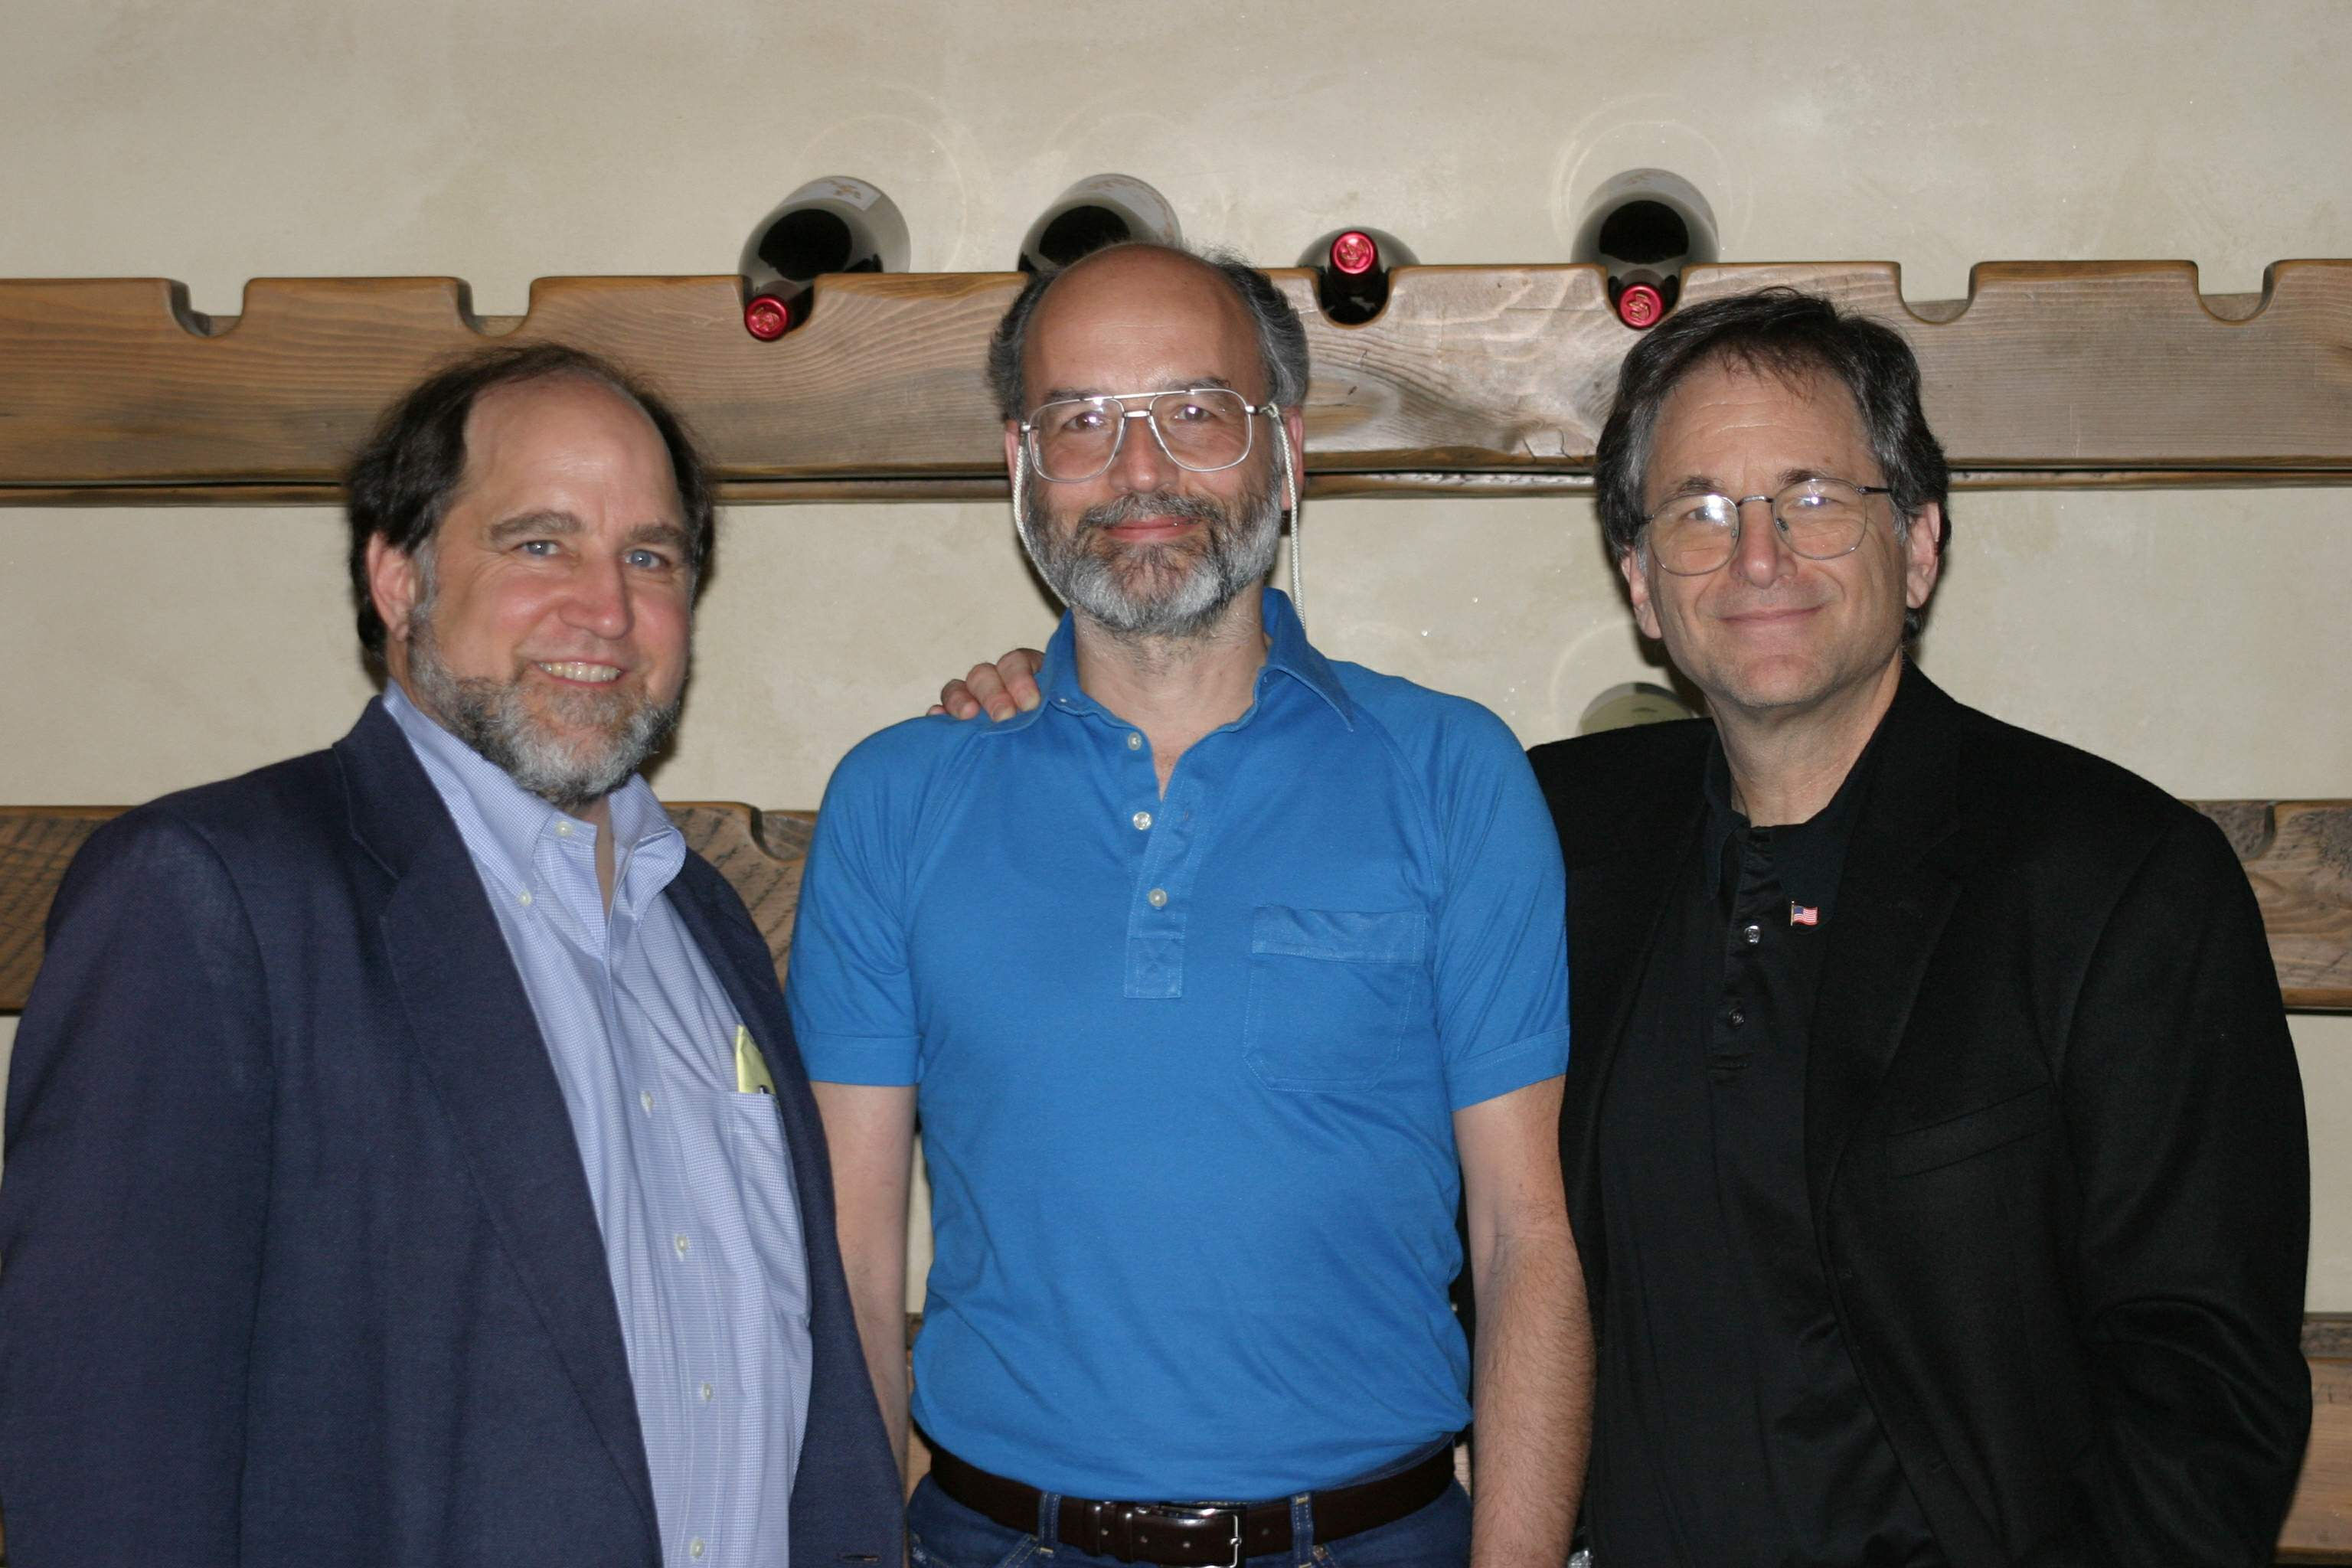
\includegraphics[height=0.15\textwidth]{RSA-2003.jpg} \\
Adi Shamir, Ron Rivest, and Len Adleman as MIT-students and in 2003\\
{\small Image credit: \url{http://www.ams.org/samplings/feature-column/fcarc-internet}, \url{http://www.usc.edu/dept/molecular-science/RSA-2003.htm}}.\\
}

\begin{exercise}[Attacks on Plain RSA]
\begin{subex}
For the RSA public key $(N,e)=(10000799791, 3)$, decrypt the ciphertext $c=1 000 000$. Can you do it without factoring $N$?
\end{subex}
\begin{subex}
Suppose we would like to use plain RSA as public-key encryption in a hybrid scheme together with AES-256 in CBC mode. We choose $N$ to have roughly 2048 bits. Use the previous subexercise to argue the insecurity of this hybrid scheme.
\end{subex}
\end{exercise}


\begin{exercise}[Perfectly secure public-key encryption?]
	Assume a public-key encryption scheme for single-bit messages with no
	decryption error. Show that, given $pk$ and a ciphertext $c$ computed via
	$c=\mathsf{Enc}_{pk}(m)$, it is possible for an unbounded adversary to determine
	$m$ with probability 1.
\end{exercise}

	
\pagebreak
\begin{exercise}[CCA security of multiple encryptions]
Claim 11.7 in [KL] states that if $\Pi=(\mathsf{Gen},\mathsf{Enc}, \mathsf{Dec})$ is a CPA-secure public-key encryption scheme for fixed-length messages, then the new encryption scheme $\Pi'=(\mathsf{Gen},\mathsf{Enc}', \mathsf{Dec}')$ with  $\mathsf{Enc}'_{pk}(m_1\|m_2\|...\|m_\ell)=\mathsf{Enc}_{pk}(m_1)\|\mathsf{Enc}_{pk}(m_2)\|...\|\mathsf{Enc}_{pk}(m_\ell)$ is CPA secure for arbitrary-length messages.

	Show that Claim 11.7 does not hold in the setting of CCA-security: Exhibit a concrete attack on a scheme $\Pi'=(\mathsf{Gen},\mathsf{Enc}', \mathsf{Dec}')$ constructed from a fixed-length CCA secure encryption scheme $\Pi=(\mathsf{Gen},\mathsf{Enc}, \mathsf{Dec})$ by defining 
\[ \mathsf{Enc}'_{pk}(m_1\|m_2\|...\|m_\ell)=\mathsf{Enc}_{pk}(m_1)\|\mathsf{Enc}_{pk}(m_2)\|...\|\mathsf{Enc}_{pk}(m_\ell) \]
\end{exercise}




\begin{bonusexercise}[El-Gamal variant]
	Consider the following public-key encryption scheme. The public key is $(G,q,g,h)$ and the private key is $x$, generated exactly as in the El-Gamal encryption scheme. In order to encrypt a bit $b$, the sender does the following:
	\begin{enumerate}
		\item If $b=0$ then choose independent random $y,z \leftarrow \mathbb{Z}_q$, compute $c_1 = g^y$ and $c_2 = g^z$, and set the ciphertext equal to $(c_1, c_2)$.
		\item If $b = 1$ then choose a random $y\leftarrow \mathbb{Z}_q$ and compute $c_1 =g^y$ and $c_2 = h^y$. The ciphertext is $(c_1, c_2)$.
	\end{enumerate}
	Show that it is possible to decrypt efficiently given knowledge of $x$. Prove that this encryption scheme is CPA-secure if the decisional Diffie-Hellman problem is hard relative to $\mathcal{G}$.
\end{bonusexercise}



\end{document}
